\chapter{Hardware and Software}
\label{hardwareandsoftware}
 
This chapter will give an in-depth look into the hardware and software used to complete the project. This knowledge is necessary to understand the design decisions made.
 
\section{Hardware}
 
\subsection{Rotary Encoder}
A rotary encoder is an electromechanical transducer to convert a rotary movement into an electrical signal. One of the most commonly used rotary encoders is the optical rotary encoder.
Its working principle is based on a Light emitting diode and a photo sensitive device, such as a photo-transistor or photo-resistor. The diode and the photo-sensitive device are located on opposite sides of a light blocking disk. This is illustrated in Figure \ref{HardEnc}.\\
The light blocking disk is perforated with small slits in a rotational symmetric and regular pattern. As soon as the disc is rotated between the diode and the photo-sensitive device, the light is transmitted and blocked in an alternating pattern.
This creates a square wave on the output of the photo-sensitive device, which frequency is dependent on the rotational speed of the disk.\cite{MotionOptischerEncoder}
 
\begin{figure}
    \begin{center}
    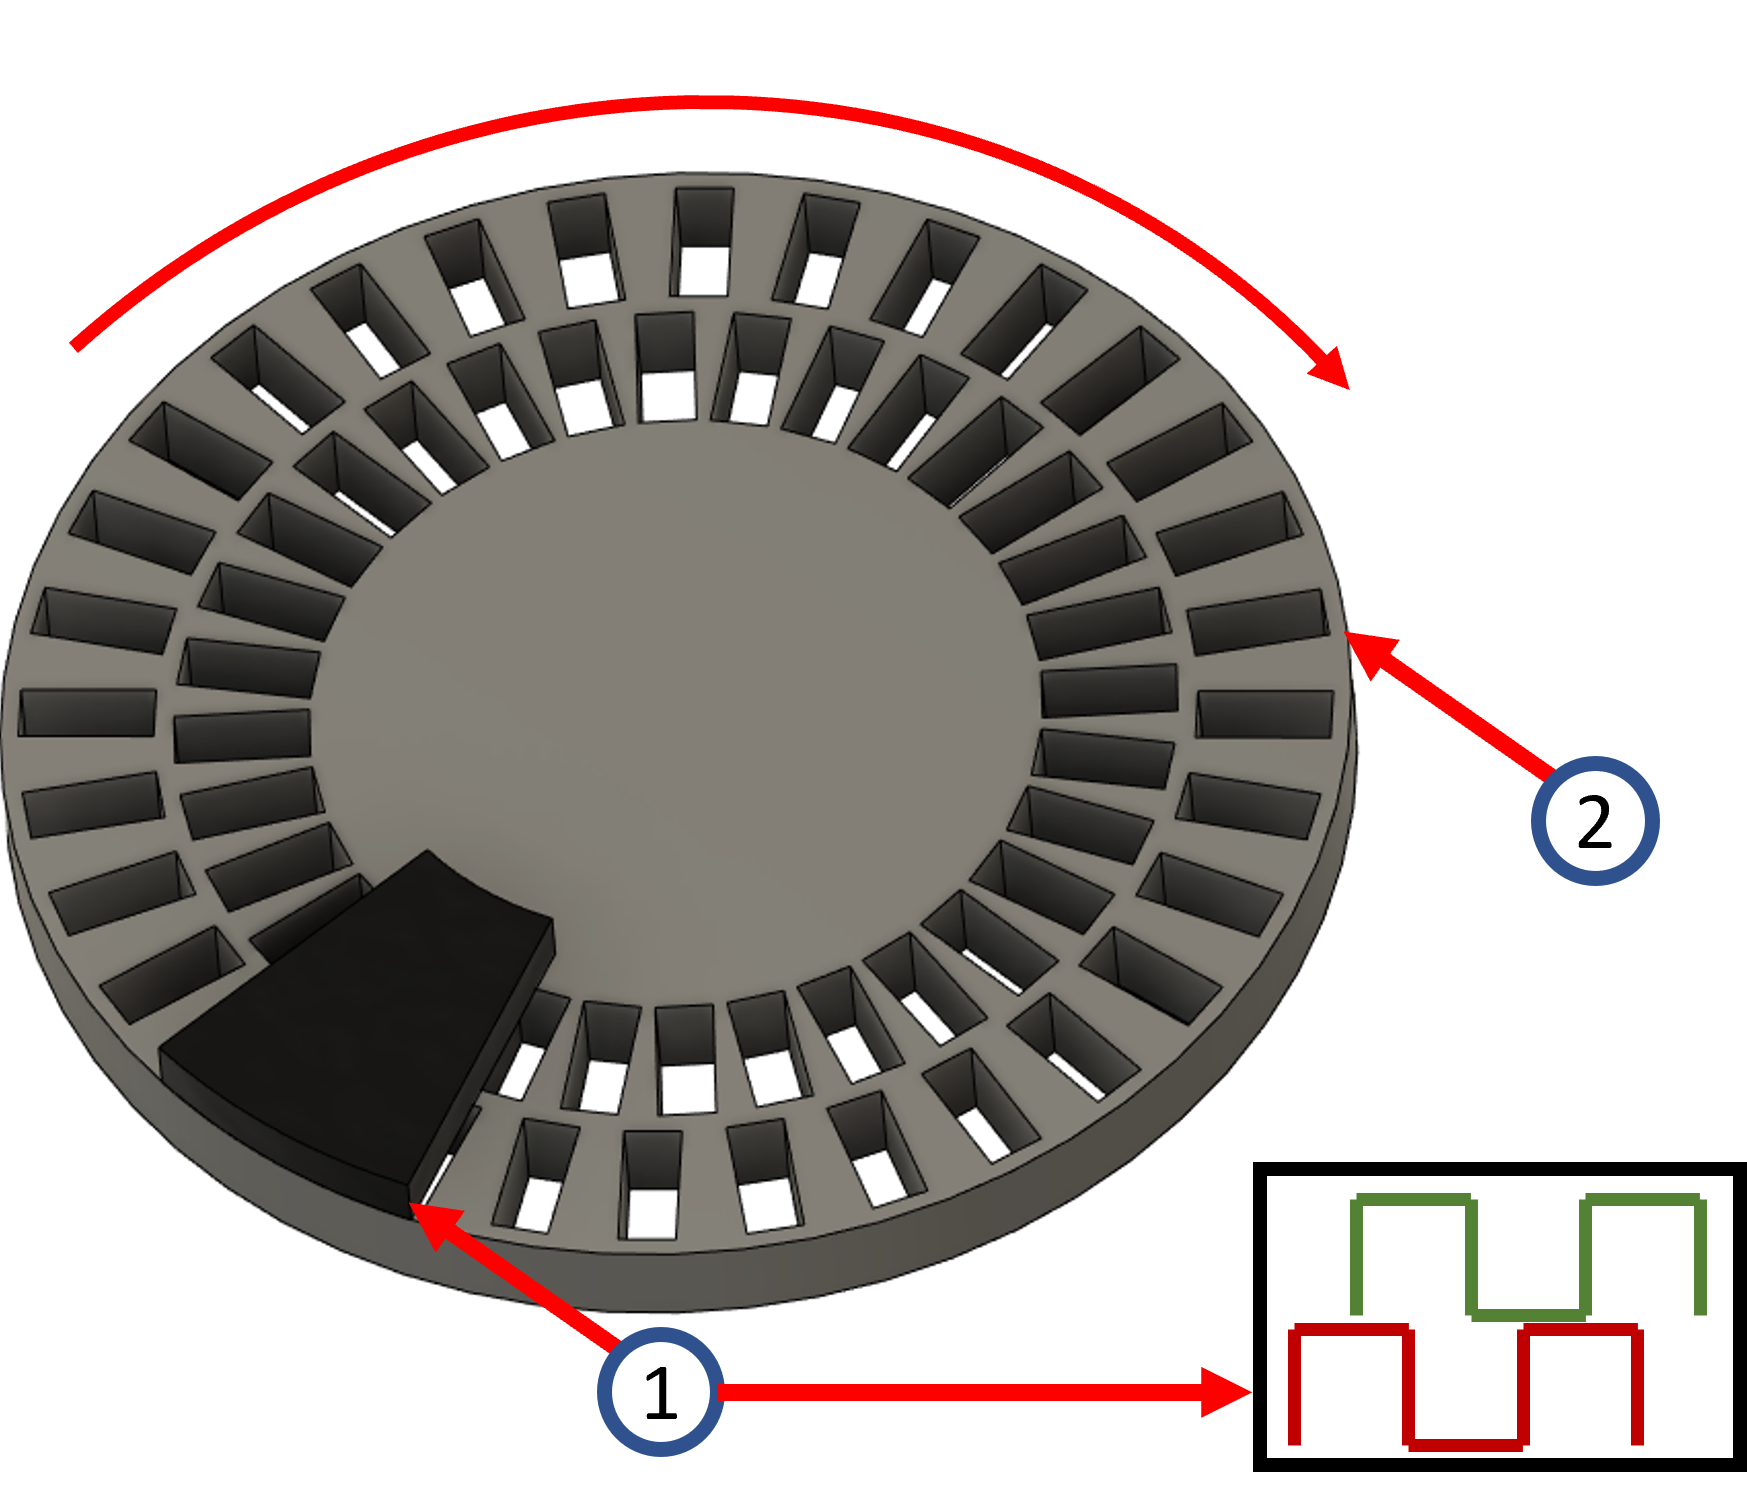
\includegraphics[width=12cm]{Pictures/HardEnc.png}
    \caption[Illustration of an optical encoder]{Illustration of an optical encoder; 1 - Detector unit and detector unit signal, 2 - Encoder disk}
    \label{HardEnc}
    \end{center}
\end{figure}
 
 
\subsection{Stepper Motors}
A stepper motor is an electrical, synchronous motor. Its rotor follows the magnetic field created in the stator exactly. In contrast to commonly known DC or AC motors, a stepper motor has a minimum angle that it needs to be rotated.
This has the big advantage, that the position is always a multiple of this angle, the so-called step angle. Therefor, a sensor is not necessary to rotate the motor by a very precise amount. A stepper motor is a cheap alternative to closed loop controlled motors. Here, an additional sensor has to determine the positional error of the motor in order to move the motor precisely.\\
The disadvantage of stepper motors usually is their low rpm limit. At a certain speed, the rotor of the motor is no longer able to follow the magnetic field created by the stator.
This can also happen when the motor is under high load. When this happens, the motor will skip steps. Therefore, stepper motors are often combined with rotational sensors in order to detect skipped steps and compensate for it.\cite{SchrittmotorenFaulhaber2022}
 
\subsection{Closed Loop Servos}
Closed Loop Servos are an electromechanical actuator with a continuous feedback loop between its output (speed, torque, position, etc…) and input (Voltage, Current).
Servos require additional electronics to compute the difference between its desired output and its current state. These electronics are typically referred to as "controller" or "driver".
Servos are used in a wide variety of mechatronic applications when high precision, reliability or dynamics are required.\cite{ServoSuh2008}
 
\subsection{Microcontroller}
A microcontroller is an integrated circuit designed to serve a specific task in a system. Microcontroller consist of a processing unit, memory as well as In- and outputs.
Within a system, a microcontroller can be used for a wide variety of tasks such as communication, data acquisition or actuator control. For mechatronic tasks, microcontrollers are commonly used as a so called embedded system.
An embedded system is designed around a microcontroller and a specific task within a project.\cite{UensalanMicrocont2022}
 
\subsubsection{TI LaunchXL F280049C}
The Texas Instruments Launchpad F280049C is a prototyping board designed around the Texas Instruments Picolo F280049C Real-Time microcontroller as an embedded system. Its design specifically targets highly dynamic control tasks while maintaining a low unit cost.
The Picolo F280049C is a 32bit floating point microcontroller with 256 KB Flash memory, 100 KB RAM and an operation frequency of 100MHz.
Further, the microcontroller has hardware support for up to two rotary encoders, a wide variety of communication protocol's as well as general purpose I/O.
In addition, the LaunchPad development board build around the microcontroller offers a debugging probe. This probe can be used to flash the microcontroller with software or observe and direct the operation of the microcontroller.
This way, it is for example possible to stop the execution of the program on the microcontroller to access and change the value of every bit in every register of the microcontroller.\cite{TILAUNCHXL}
 
\subsubsection{Logic Level Shifter}
A logic level shifter is an electronic circuit designed to convert one logic voltage level into another one, while maintaining the signal integrity. In modern mechatronic systems, it is often necessary that different electronic systems can communicate with each other. In some cases, however, it is not possible that all components work on the same voltage level. This makes it inevitable to use a logic level shifting circuit.\cite{berle2018tabellenbuch}
 
 
\subsection{Raspberry Pi}
A Raspberry Pi is a Single board computer that features a full graphic operating system based on Linux. Further, it offers wireless connectivity as well as general purpose I/O's. The Raspberry Pi is mostly open source and very cost-effective. Because it has a very wide customer base, the Raspberry Pi has a wide variety of hardware and software add-ons available.\cite{RaspberryPiFoundation}
%%TODO Bild??
 
\section{Software}
\subsection{Matlab and Matlab-Simulink}
MATrix LABoratory (MATLAB) is an Integrated Development Environment (IDE)
and programming language. MATLAB was developed in the need of a numerical algebraic
system at the university of New Mexico. On this base, the company MathWorks (see
\ref{AppendixListOfCompanies}) was created. Since 1984 MathWorks is further developing MATLAB and
additional software for numerical algebraic computing. To support different hardware
packages MathWorks offers so-called toolboxes. These toolboxes contain functions and
scripts for communication, data acquisition, motion control etc.
MATLAB is mainly used in technical development and research.\cite{Mathworks}
 
\subsection{Programing Language C}
C is a high level programming language. It is most commonly used to write applications for embedded systems. It is chosen over low level programming languages
such as Assembly because of the increasing complexity of programs for embedded systems. C is a compiled programming language. This means that a program needs to be translated (compiled) to machine code before it can be executed.
This translation is done with a program called "compiler". Compared to lower level languages such as Assembly, the code reusability of C has proven to be a step forward in the development of embedded systems.\cite{ISO2022}
 
 
\subsection{Programing Language Python}
Python is a high level object-oriented programming language. In contrast to C, Python is an interpreted language. This means, an Interpreter translates source code into machine commands in
real time, while the program is executed. Python features a good combination of capability and ease of uses. This makes the language easy to learn for beginners while remaining very powerful.
Python further features a huge variety of proprietary and community build support packages and is based on the one of the most used programming languages used today.\cite{PythonFoundation2022}
 
\subsubsection{Kivy}
Kivy is an open source Python library for the rapid development of graphical user interfaces and apps. It is script based and its scripting language can be directly implemented in Python. Further, Kivy supports use with touch screens. During this project, Kivy was used in order to develop the software for the Human Machine Interface.\cite{Kivy.org2022}
 
 
\subsection{Code Composer Studio}
Code Composer Studio is an Integrated Development Environment produced by Texas Instruments. It presents an interface to the Hardware produced by Texas Instruments and offers optimizing compilers for C and C++. Further, Code Composer Studio features support packages for the development and deployment of software to Texas Instruments Hardware, such as the TI LaunchXL F280049C. These support packages, in combination with a hardware debugging probe, enable the programmer to interact with the processor in real time.\cite{Instruments2022}
 
 
\subsection{Git}
Git is a software tool for source code management and versioning, as well as for parallel development. Git was developed by Linus Torvald in 2005. Git was developed in the need of source code management software for the development of the operating system Linux. Git allows development in so-called branches. These are independent copies of an already existing and probably used software. This ensures that modifications or enhancements are not affecting already used software. If a feature is finished, it can be merged back into the higher-level branch. Merging is the process of bringing two files, directories or branches together. Different developers, working on different features of the same project, is called parallel development. Further, Git is a tool for software versioning. Software versioning is a tracking of changes in a project. In case of a mistake, the project can be recovered to every tracked point.\\
During this project, Git was very heavily used for software versioning as well as backup tool. This way, it was possible to revert changes to the software with very little work.
 
 

